\documentclass{article}
\usepackage[utf8]{inputenc}
\usepackage{enumitem}
\usepackage{listings}
\usepackage{amsmath,amssymb}
\usepackage{geometry}
\usepackage[T1]{fontenc}
\usepackage{graphicx}


\geometry{
 a4paper,
 left=38mm,
 right=38mm,
 top=38mm,
 bottom=38mm
 }

\lstset{
    language=C,
    showstringspaces=false,
    breaklines=true
}



\title{ME 333 Homework 6}
\author{Marshall Johnson}
\date{February 15, 2022}

\begin{document}

\maketitle

\section*{Chapter 24 LED Project}

\begin{enumerate}[label=\textbf{24.1.2})]
    \setcounter{enumi}{2}
    \item \textbf{Choose $R$} \\
    
    10k$\Omega$

\end{enumerate}

\begin{enumerate}[label=\textbf{24.2.1})]
    \item \textbf{PWM Calculation} \\
    
    PR3 should be 3999.
    
    $$50000 = (P + 1) * 1 * 12.5 \text{ns}$$
    $$\therefore P = 3999$$ \\

\end{enumerate}

\begin{enumerate}[label=\textbf{24.2.2})]
    \item \textbf{PWM Program} \\
    
    Screenshot files with description:

    \begin{enumerate}
        \item OC1\_waveform.png: the OC1 waveform. \\
        
        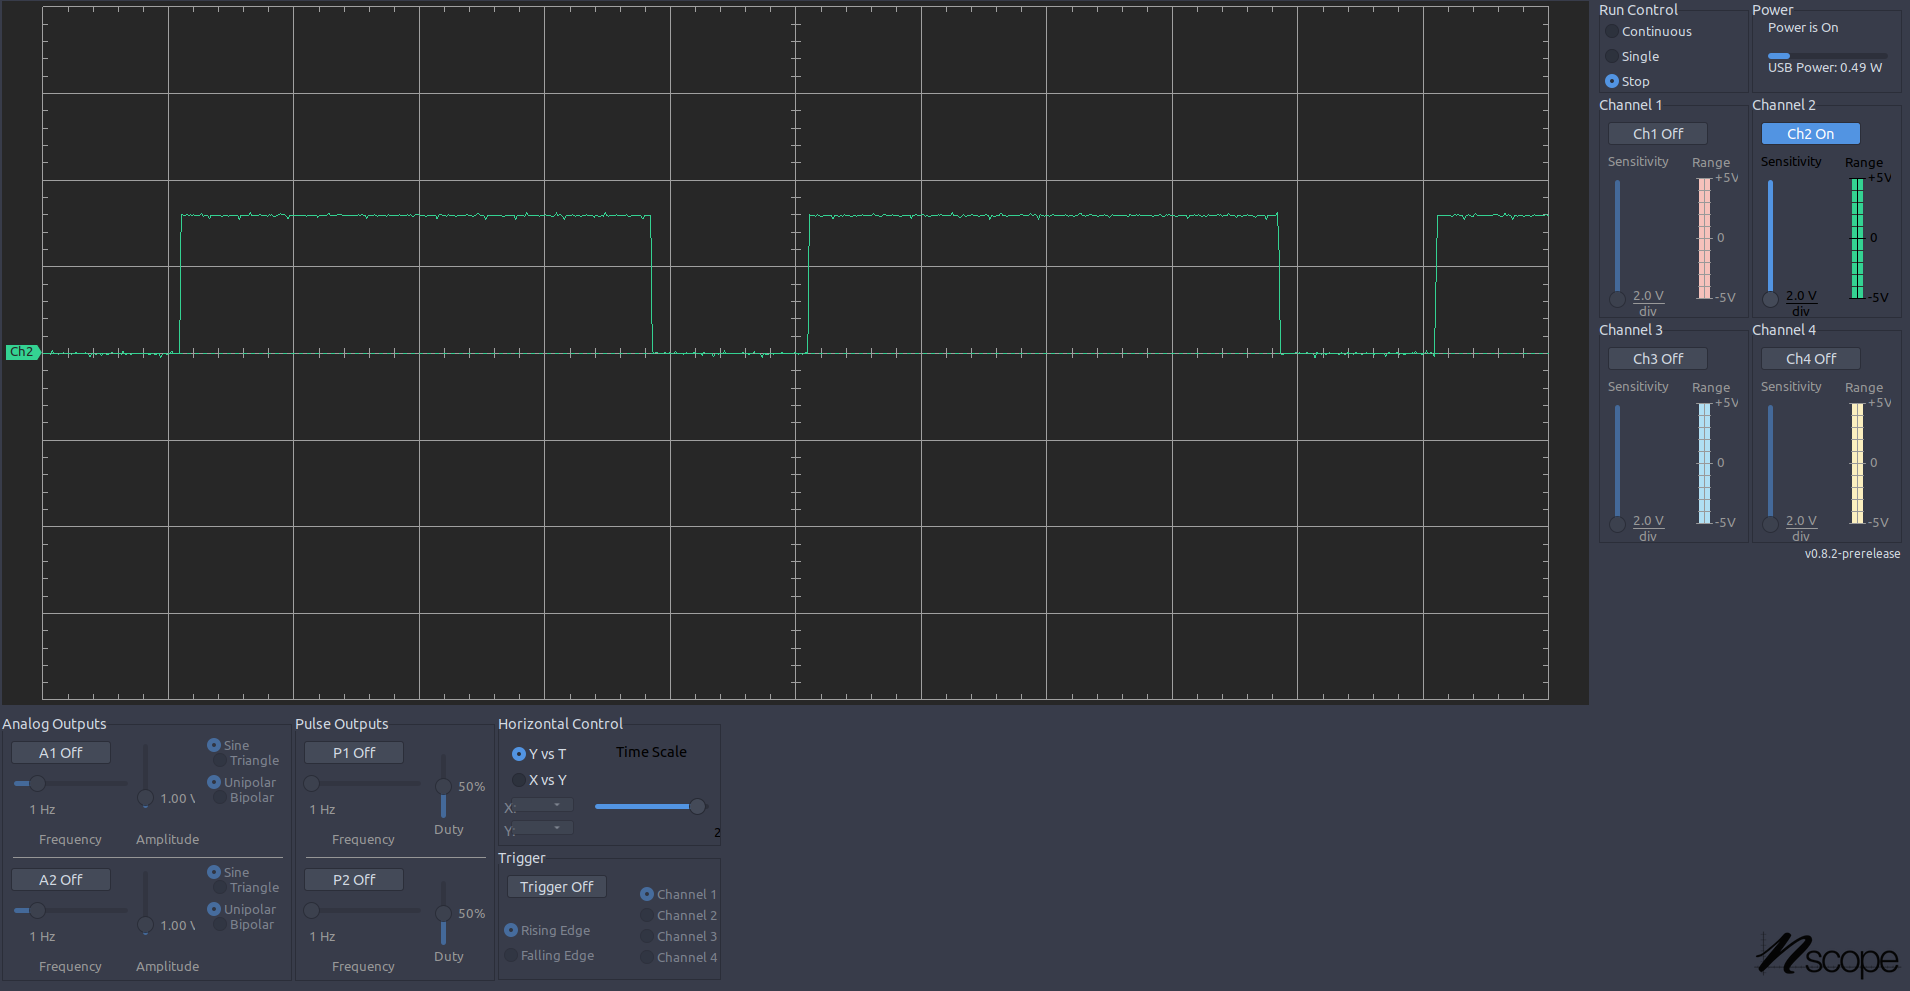
\includegraphics[width=\linewidth]{OC1_waveform.png}
        \pagebreak
        \item Vout.png: sensor voltage with capacitor in circuit \\
        
        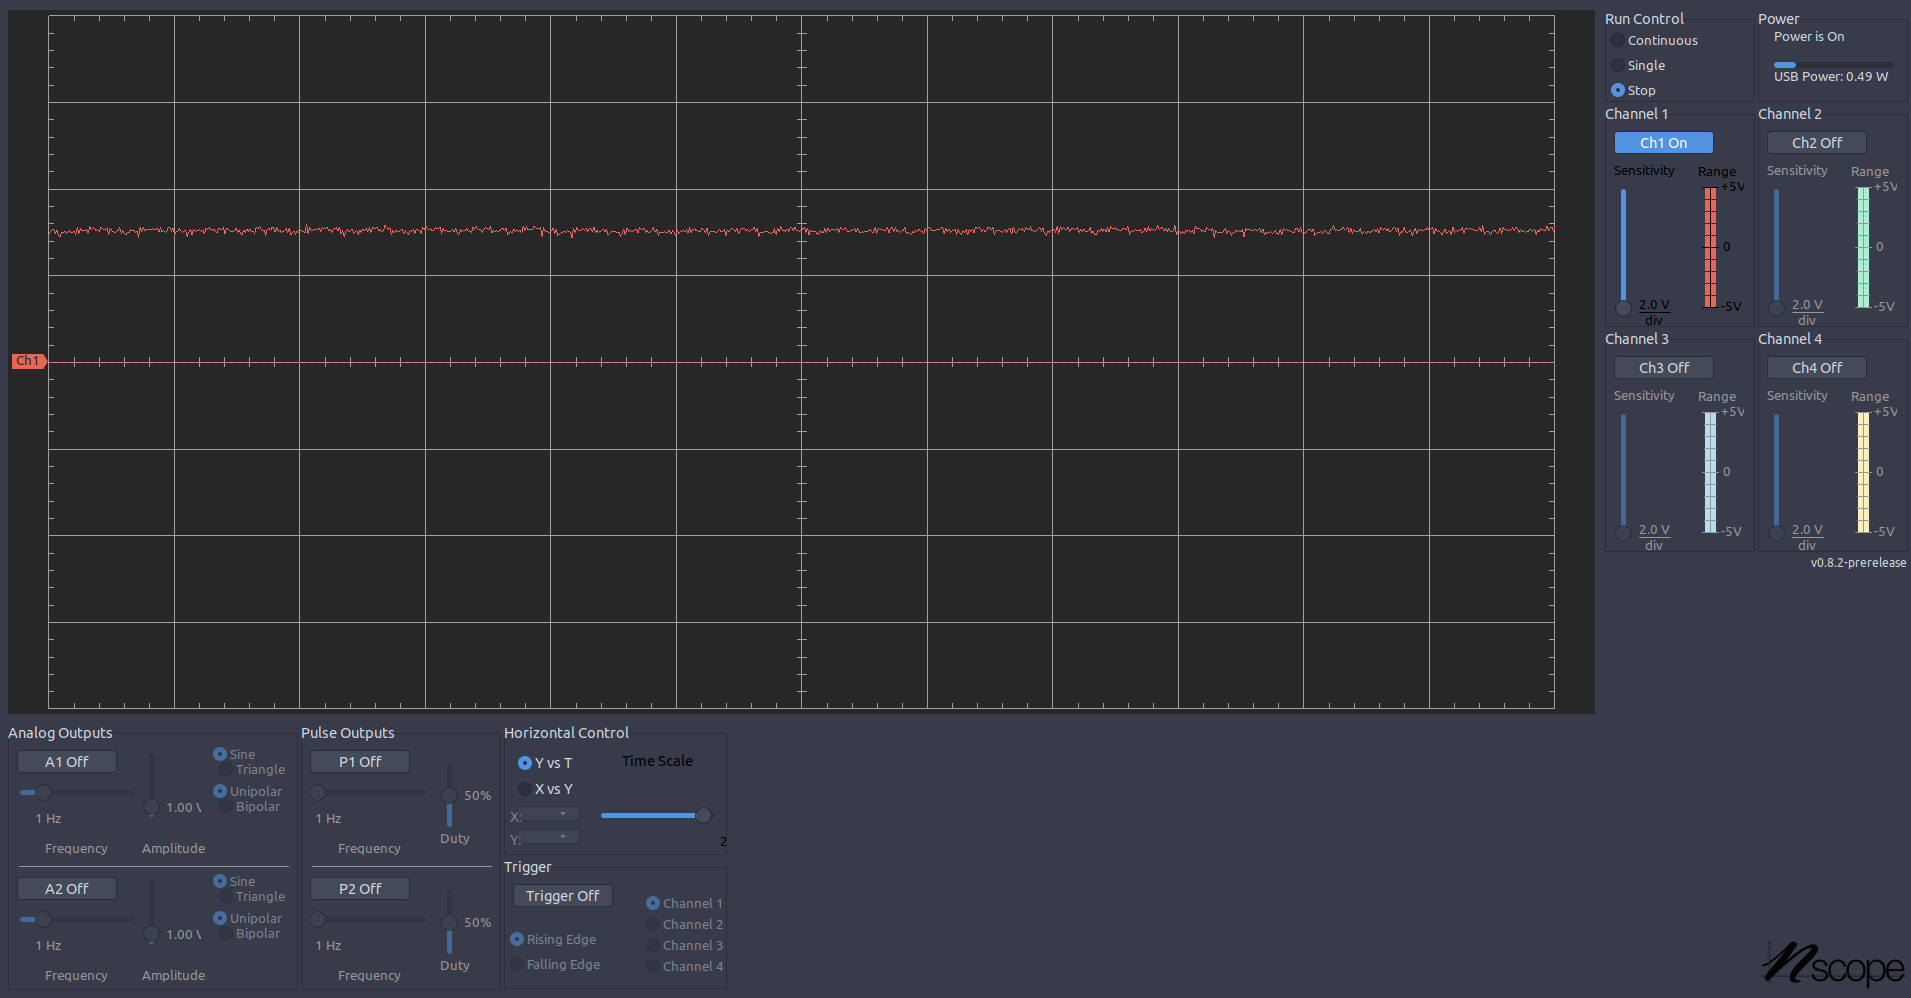
\includegraphics[width=\linewidth]{Vout.png}
        \item Vout\_nocap.png: sensor voltage without capacitor in circuit \\
        
        \includegraphics[width=\linewidth]{Vout_nocap.png}
    \end{enumerate}

\end{enumerate}

\pagebreak
\begin{enumerate}[label=\textbf{24.3.1})]
    \item \textbf{Get a screenshot of your oscilloscope trace of V out showing 2-4 periods of what should be
    an approximately square-wave sensor reading.} \\
    
    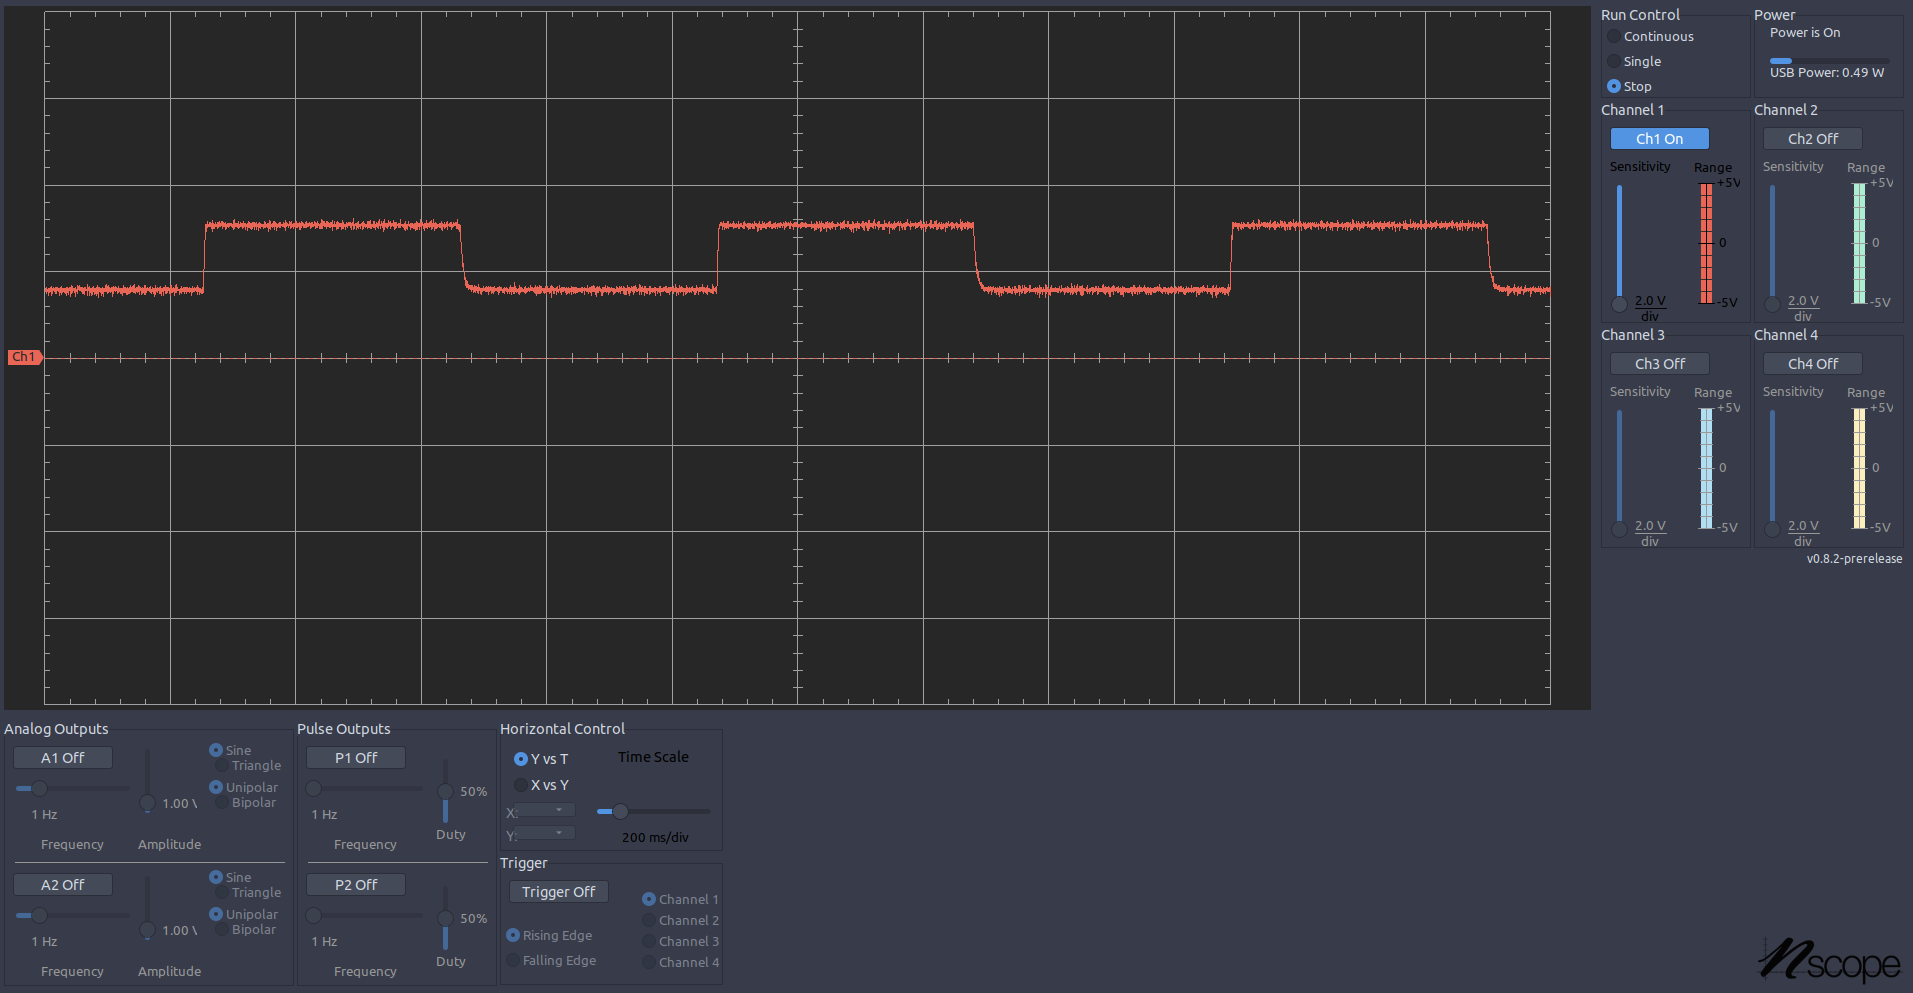
\includegraphics[width=\linewidth]{Vout_trace_dim.png}

\end{enumerate}

\begin{enumerate}[label=\textbf{24.3.2})]
    \item \textbf{Turn in your code.} \\
    
    See pwm.c
    
\end{enumerate}

\end{document}
